\subsection{\glsentryshort{gps}}
A commonly used system for location estimations are the \gls{gps}. \gls{gps} uses satellites to estimate speed and location, by utilizing the \gls{toa} method \cite{web:GPSUseTOA}. The \gls{gps} locator has to be placed on the drone and the coordinates have to be communicated wirelessly to the ground station.

The available drone (3DR Solo) has an integrated \gls{gps} module on-board, UBLOX Neo m7n. Users of this drone have 
experienced long satellite acquisition times, it usually takes 30 seconds to require a position on known area and up to one minute if the drone is flying in new areas \citep{datasheet:NEO7}. %The problem with this long satellite acquisition time is caused by the copper foil that are protecting the \gls{gps}. It may interferes with the electronic and can create shortcuts on the board if the copper foils isn't applied properly\citep{News:3DRGPS}. 

The precise accuracy of the \gls{gps} standard cannot be generalised, because its precision depends on many varying parameters. The U.S government however promises a worst case pseudorange (Pseudorange is the distance from the \gls{gps} satellite to the \gls{gps} device) accuracy of 7.8 meters at a 95\% confidence level, this means that the distance from a GPS satellite to a receiver have an accuracy of at least 7.8 meters for more than 95\% of the time \citep{web:USofAsGPSAccuracy}. 

The actual end user accuracy of the \gls{gps} is frequently being measured by the \gls{ffa}, their last tests show that the end user should normaly expect between 3-8 meters accuracy without the use of any augmentation systems. However in some cases, a range error of up to 23 meter was registered \citep{web:FFAGPSAccuracy}.

If the drone is \SI{120}{\meter} from the ground station, and the drones position is found, but with a deviation of 3 meters, that result in the angle of the motor stand have an error of $\theta = \arctan\left(\frac{3}{120}\right) = \SI{24.995}{\milli\radian}$. This means that the \glossary{gps} method is not meeting the required precision found in \autoref{sec:RequiredPrecision} \autoref{eq:RequiredPrecision}, and is therefore not feasible for the purpose of the project. 

If \gls{gps} is combined with some augmentation systems it is possible to have a higher accuracy. Examples of augmentation systems could be to use other wireless signals to position the user, such as wifi and cellular signals. 

With the limited and varying precision of the \gls{gps} method, it is not able to deliver the needed accuracy for this project, therefore the method is discarded, and is therefore not investigated further.  

\subsection{Radar}
When tracking objects an obvious mention is radar technology. Radars is used extensively around the world for geological observation, general surveillance and detection and tracking of flying objects such as airplanes and missiles \citep{radar_handbook}. 
Radar detection and tracking works by having a radar station transmitting a beam of microwave-frequency electromagnetic waves in the direction of an object. When the beam hits an object the waves are reflected back to the radar station. The time from transmission to reception is then used to find the distance to the target, and combined knowledge of the radars azimuth and elevatory heading the targets direction can be deduced, thus the target is located \citep{TechReport:RadarSystem}.

An illustration of a radar emitting a signal which is reflected upon a plane is seen on \autoref{fig:RadarMethodDrawing}. 
\begin{figure}[h!]
    \centering
        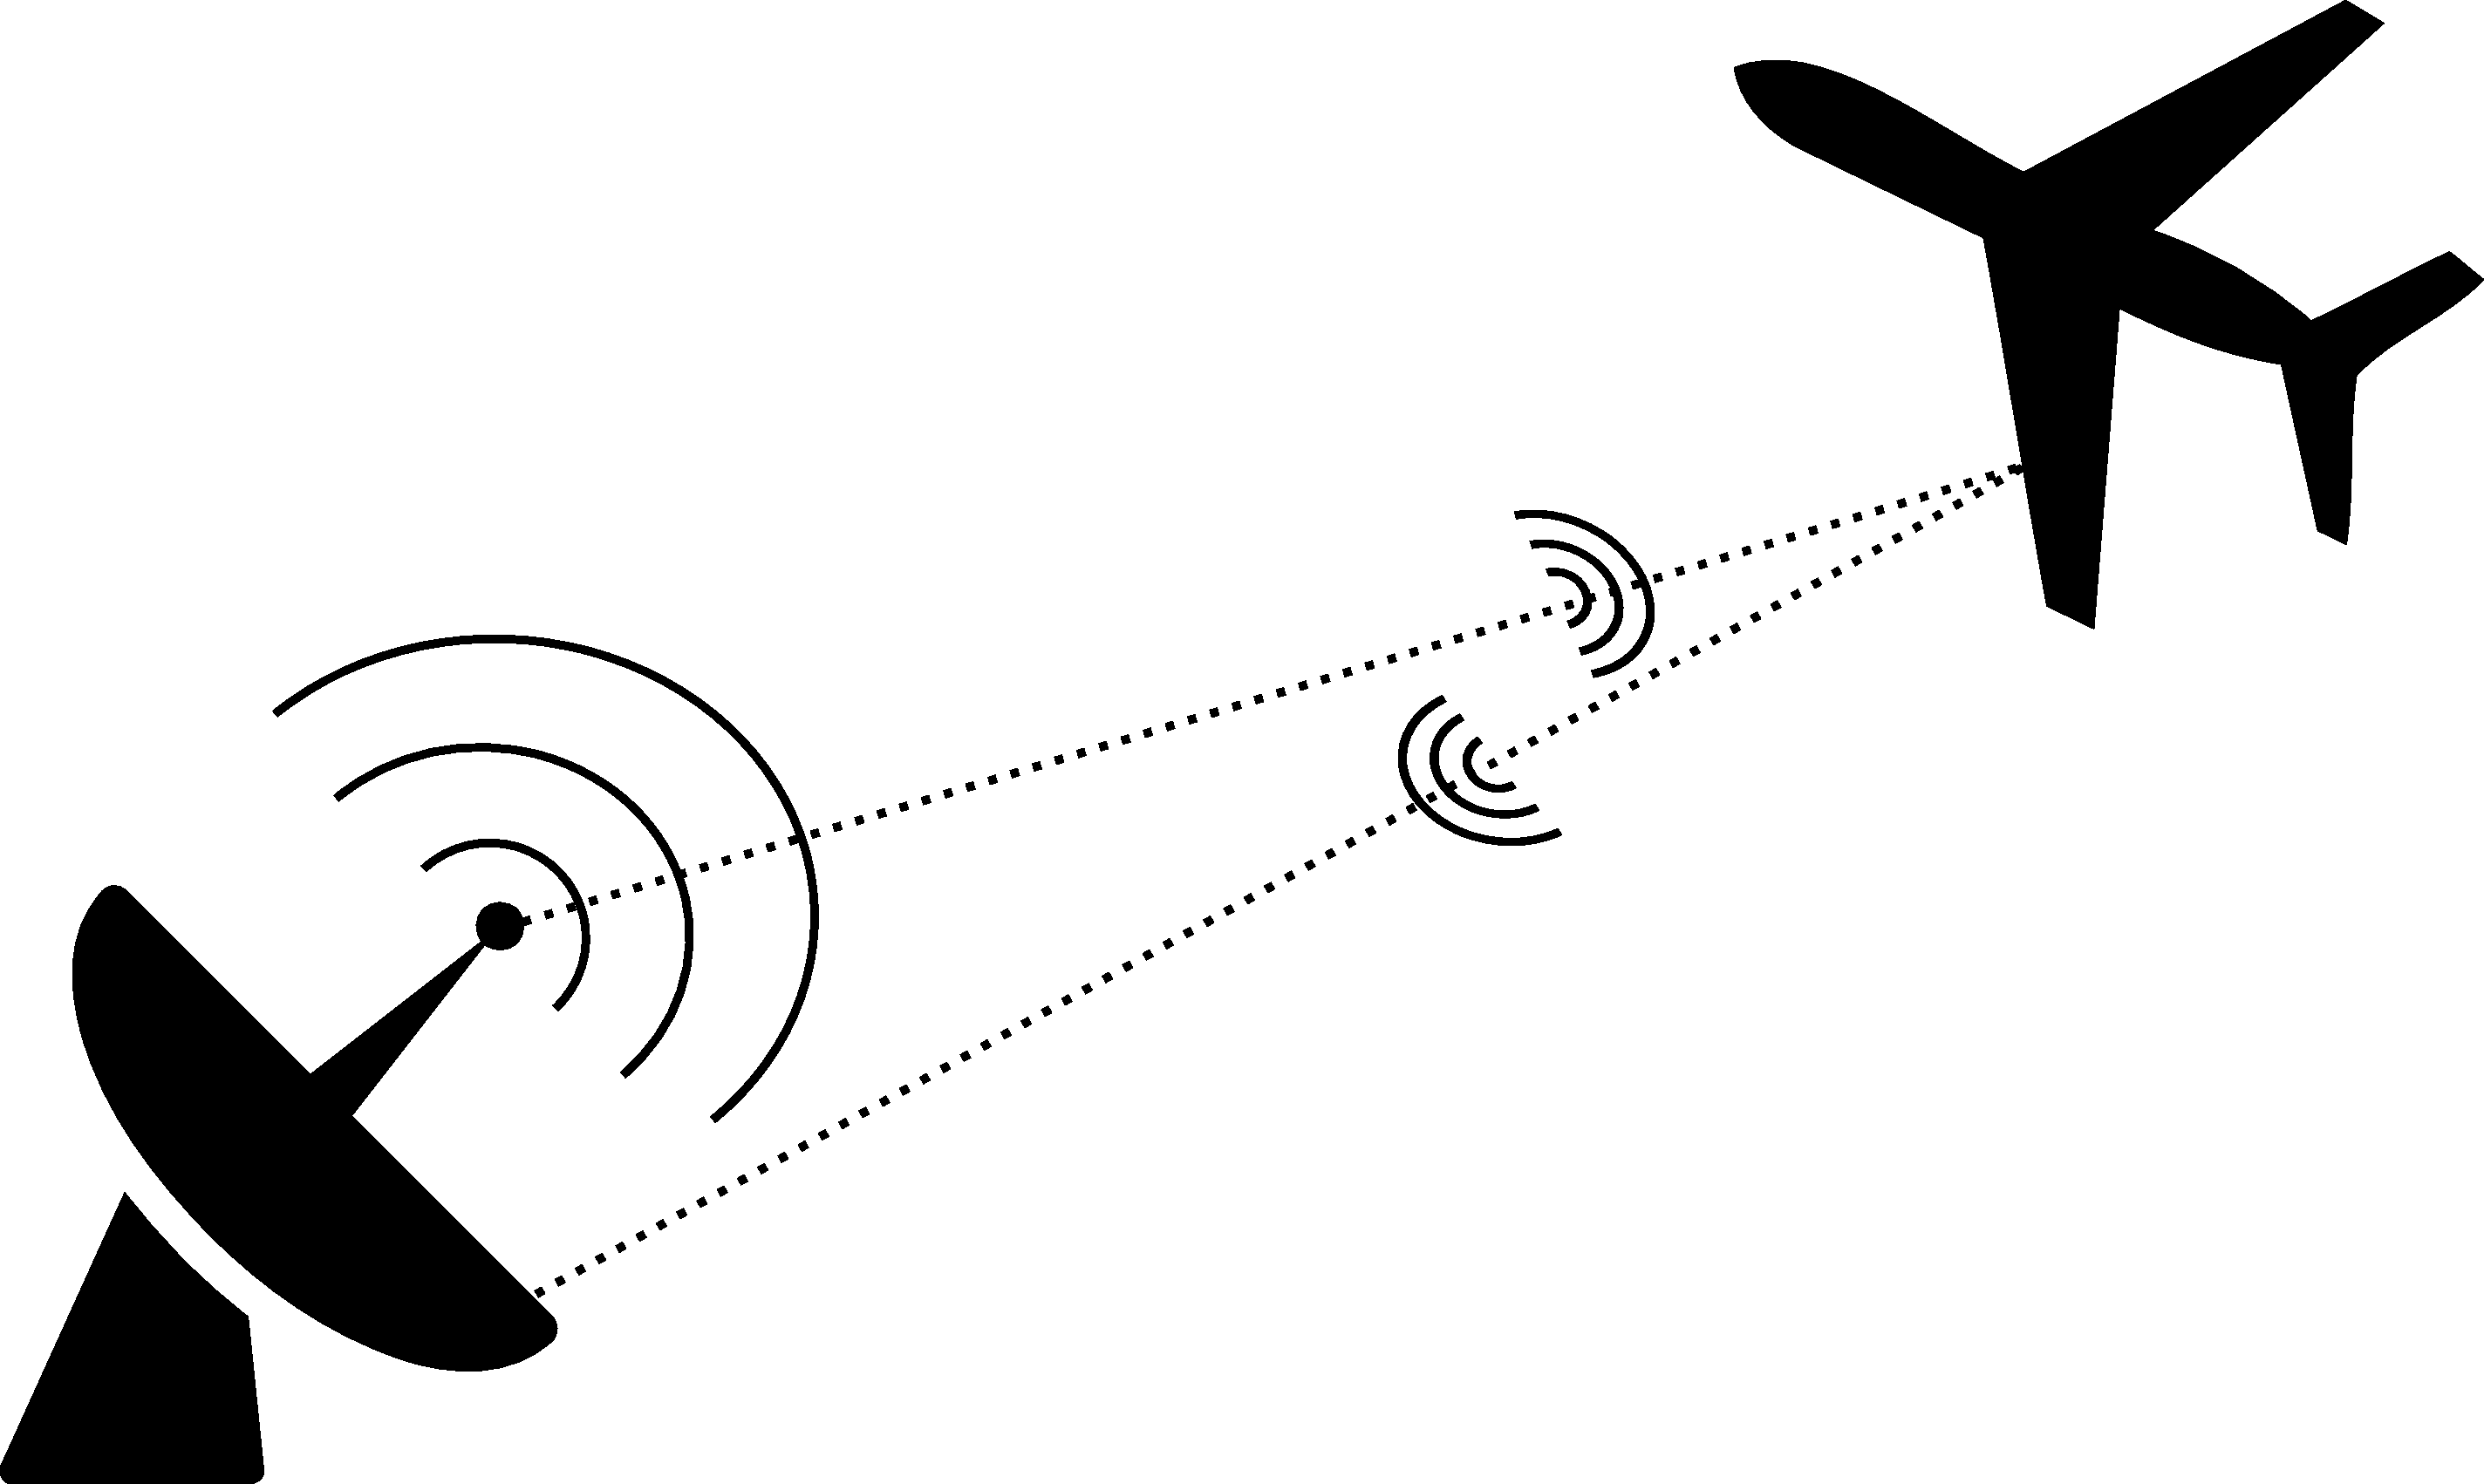
\includegraphics[width=0.5\textwidth]{figures/tracking/RadarMethodDrawing.pdf}
        \caption{The radar emitted an electromagnetic wave. The wave hits a plane, and is reflected back to the radar.}
        \label{fig:RadarMethodDrawing}
\end{figure}

\newpage
Many types of radar exists. When used for geological observation a wide beam is desirable, when used for aircraft or missile detection full $360\degree$ view is needed and when used for tracking a single targets speed and heading a very narrow beam is desired \citep{radar_handbook}.

\autoref{eq:Radar:ThinkItIsTheFrissGuyAgain} is the radar equation, it can be used to estimate the signal strength of the received reflections \citep{web:ThroughTheEyesOfARadar}. 
\begin{equation} \label{eq:Radar:ThinkItIsTheFrissGuyAgain} 
P_{r} = P_{t} \cdot  \frac{G_{r} \cdot G_{t} \cdot  \lambda^{2} \cdot \sigma}{(4\pi)^{3} \cdot R_{t}^{2} \cdot R_{r}^{2}} \addunit{\watt}
\end{equation}
\startexplain
\explain{$P_{r}$ is the power received}{\si{\watt}}
\explain{$P_{t}$ is the power transmitted}{\si{\watt}}
\explain{$G_{r}$ is the gain of the receiver antenna}{\si{1}}
\explain{$G_{t}$ is the gain of the transmitter antenna}{\si{1}}
\explain{$\lambda$ is the wavelength}{\si{\meter}}
\explain{$\sigma$ is radar cross-section (RCS)}{\si{\meter^2}}
\explain{$R_{t}$ is the distance between the transmitter antenna and the object}{\si{\meter}}
\explain{$R_{r}$ is the distance between the receiver antenna and the object}{\si{\meter}}
\stopexplain

\autoref{eq:Radar:ThinkItIsTheFrissGuyAgain} can be simplified by assuming that the receiver and the transmitter is the same antenna, and that it has a gain of 1.
\begin{equation} \label{eq:Radar:simplyfiedEquation1} 
P_{r} = P_{t} \frac{\lambda^{2} \sigma}{(4\pi)^{3} R^{4}} \addunit{\watt}
\end{equation}

By assuming a frequency of \SI{800}{\mega\hertz} and a distance between the antennas and the drone of \SI{120}{\meter} then \autoref{eq:Radar:simplyfiedEquation1} becoms: 
\begin{equation} \label{eq:Radar:simplyfiedEquation3} 
P_{r} = P_{t} \cdot \sigma \cdot 341.280 \cdot 10^{-15} \addunit{\watt}
\end{equation}

The radar cross-section of a drone is estimated to be between -10 to \SI{5}{\deci\belsm} (Where \SI{-10}{\deci\belsm} is the equivalent of a stealth military aircraft and \SI{5}{\deci\belsm} is a medium sized commercial aircraft) \citep{web:ThroughTheEyesOfARadar}. 

%Thus the radar cross-section, $\sigma$, of a drone is between $10\dfrac{-10}{11} = 0.1$ and $10\dfrac{5}{10} = 3.1623$

By including the radar cross-section of a medium sized commercial aircraft, to serve as a best case scenario in \autoref{eq:Radar:simplyfiedEquation2}, the received power can be calculated by \autoref{eq:Radar:simplyfiedEquation2}.
\begin{equation} \label{eq:Radar:simplyfiedEquation2} 
P_{r} = P_{t} \cdot 10^{\frac{5}{10}} \cdot 341.280 \cdot 10^{-15} = P_{t} \cdot 1.079 \cdot 10^{-12} \addunit{\watt}
\end{equation}

From \autoref{eq:Radar:simplyfiedEquation3} it is seen that if the used antenna does not have any gain, and if the target object has a radar cross-section of \SI{5}{\deci\belsm}, one needs to transmit approximately $10^{12}$ times more power than one needs to receive. 

If a received power of \SI{-20}{\deci\belm} is desired, \autoref{eq:Radar:simplyfiedEquation3} can be used to calculate the needed transmission power, as seen in calculated in \autoref{sec:radarRequiredPower2}
\begin{subequations}
\begin{align}  
P_{r} &= P_{t} + 10\cdot \log_{10}\left(1.079 \cdot 10^{-12}\right) \notag \\ 
P_{t} &= \SI{100}{\deci\belm} \label{sec:radarRequiredPower2}
\end{align}
\end{subequations}

The power needed decreases with increased gain. Using the exact radar cross-section of the target in question is probably mean a decreased efficiency, due to the radar cross section of the target being smaller than the assumed \SI{5}{\deci\belsm}. 

High gain antennas are needed in order for the radar method to work, because it is assumed that the required power levels described by \autoref{sec:radarRequiredPower2}, is not feasible for this project. Antennas with high a gain is outside the scope of this project and therefore this method is not possible for this project.

%with a limited transmission power of  the the needed gain can be found by looking back at \autoref{eq:Radar:ThinkItIsTheFrissGuyAgain}, as seen in \autoref{eq:RadarNeededGain}. 
%\begin{subequations}
%\begin{align} 
%&G_{r} \cdot G_{t} \cdot 1.079 \cdot 10^{12}\cdot P_t = P_r  \label{eq:ExplainNextEq}\\
%&\implies G_{r} \cdot G_{t} \cdot 1.079 \cdot 10^{-12} = 1 \label{eq:RadarNeededGain}\\
%&\implies G_{r} \cdot G_{t} = 0,927 \cdot 10^{12} \label{eq:RadarNeededGain3}
%\end{align}
%\end{subequations}
%
%\autoref{eq:RadarNeededGain3} can be simplified to \autoref{eq:RadarNeededGain2}, by assuming that $G_{r} = G_{t}$. \autoref{eq:RadarNeededGain2} calculates the needed gain for each of the two antennas. 
%\begin{align} \label{eq:RadarNeededGain2} 
%G_{r} \wedge G_{t} = \sqrt{0,927 \cdot 10^{12}} = 0.963 \cdot 10^6 \\
%G_{r} \wedge G_{t} = 10 \log10(0.963 \cdot 10^6) =  \SI{59,835}{\decibel}
%\end{align}

%As it is seen in \autoref{eq:RadarNeededGain2} the radar detection method needs two antennas with at very high gain. Antennas with this high a gain is outside the scope of this project and therefore this method is not possible for this project. 
